\section{Definicja wymagań}
Celem tej części projektu było zaprojektowanie i napisanie oprogramowania robota.
Określono, że będą dwa rodzaje aktorów ludzkich wchodzących w interakcje z systemem:
\begin{itemize}
    \item administrator -- jest tylko jeden i ma dostęp do wszystkich ustawień i zarządzania pozostałymi użytkownikami;
    \item pracownik ochrony -- ma dostęp do kluczowych funkcjonalności;
\end{itemize}
Funkcjonalności, jakie ma posiadać system zostały zdefiniowane na diagramie przypadków użycia \ref{rys:usecases}.
\begin{figure}[!hb]
    \centering 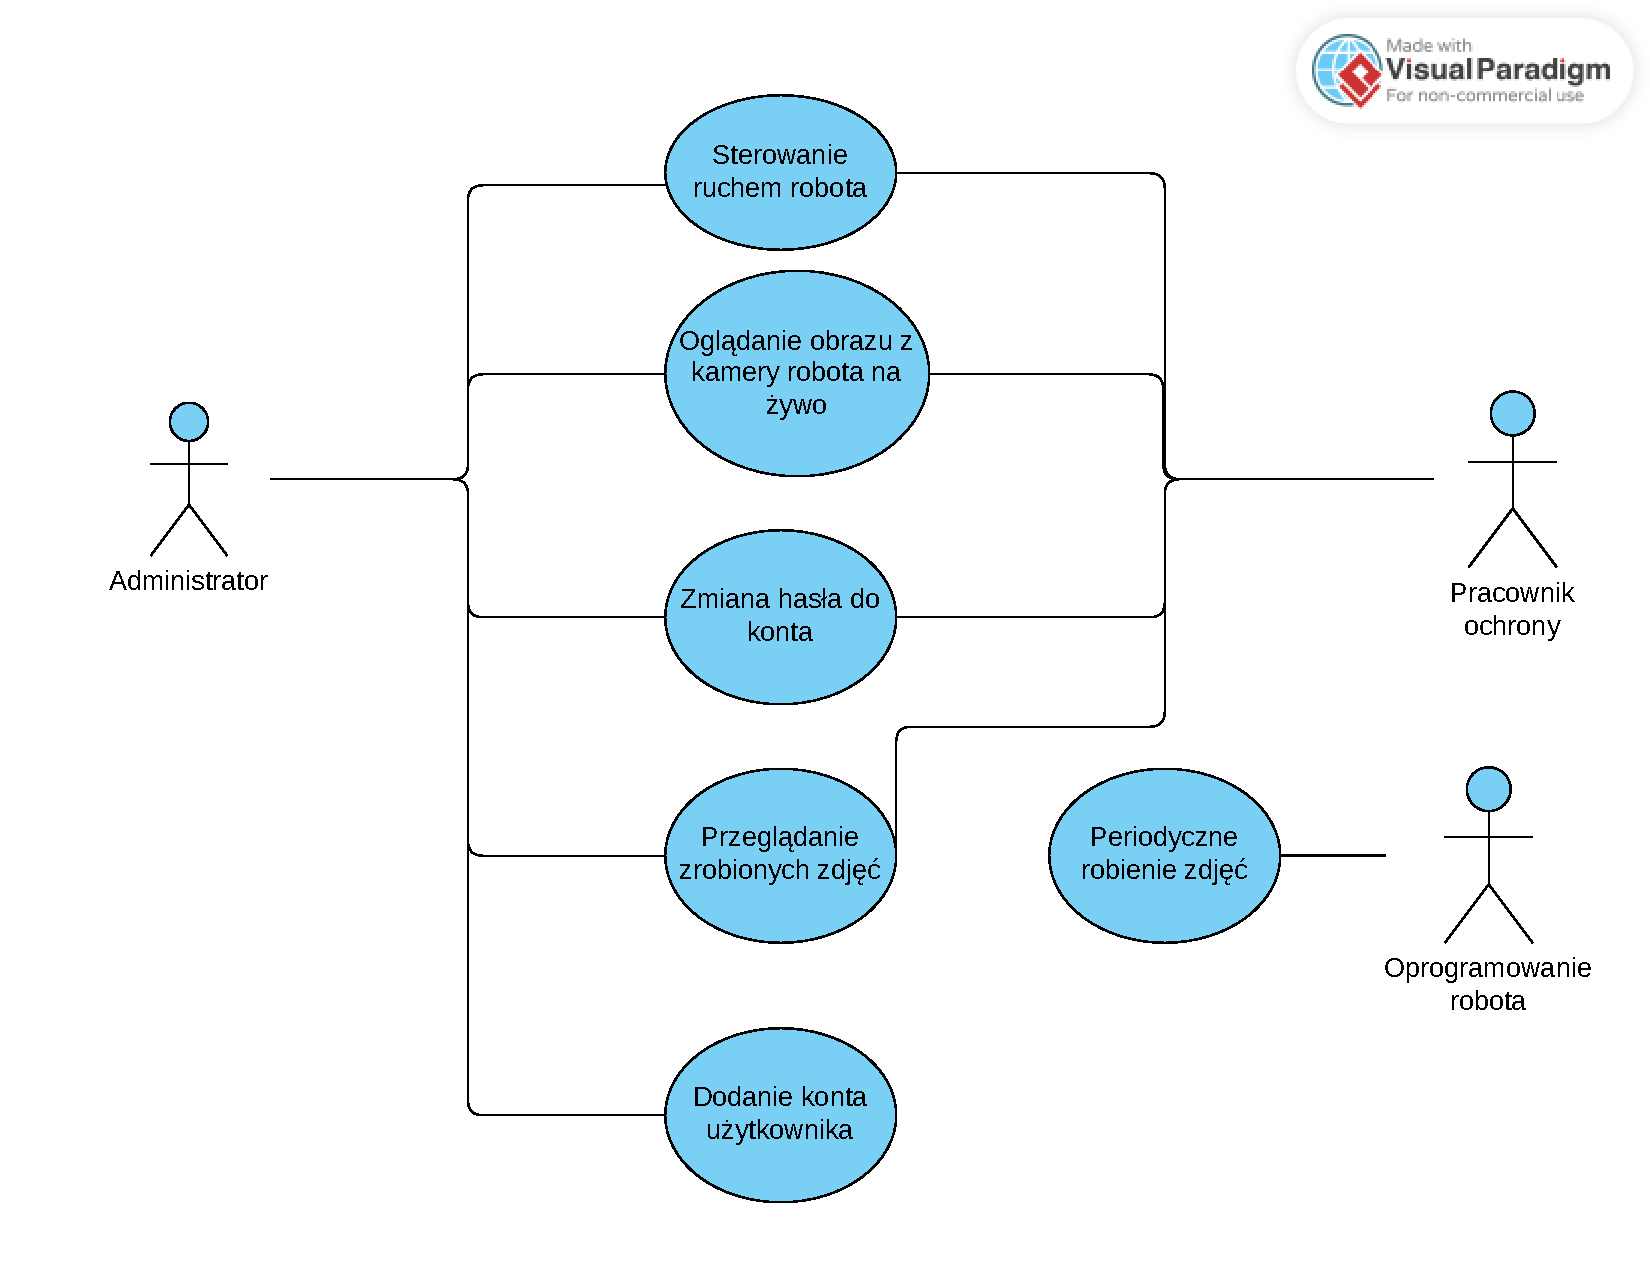
\includegraphics[width=1.0\linewidth]{robot_usecases.pdf}
    \caption{Diagram przypadków użycia}
    \label{rys:usecases}
\end{figure}

\section{Architektura systemu}
Zdecydowano się na interfejs użytkownika w formie aplikacji przeglądarkowej (webowej).
Rozwiązanie to pozwala na dostęp do systemu bez instalacji żadnego oprogramowania.
Ponadto taka forma aplikacji pozwala na dostęp przez szeroką gamę urządzeń końcowych -- komputery, smartfony, tablety itp.

Zgrubny podział aplikacji jest na:
\begin{itemize}
    \item Frontend \\
    Aplikacja uruchamiana w przeglądarce użytkownika.
    Prezentuje dane przychodzące z robota użytkownikowi.
    Przesyła do backendu dane pochodzące od użytkownika.
    \item Backend \\
    Aplikacja działająca na sprzęcie robota.
    Wysyłająca dane do frontendu i przetwarzająca przychodzące dane.
    Steruje zachowaniem robota.
\end{itemize}

Na backendzie ze względu na różnorodną i wielowarstwową funkcjonalność aplikacji zdecydowano się na architekturę mikroserwisową.
Wysokopoziomowa komunikacja modułów między sobą ukazana jest na diagramie komponentów \ref{rys:components}.
\begin{figure}[!hb]
    \centering 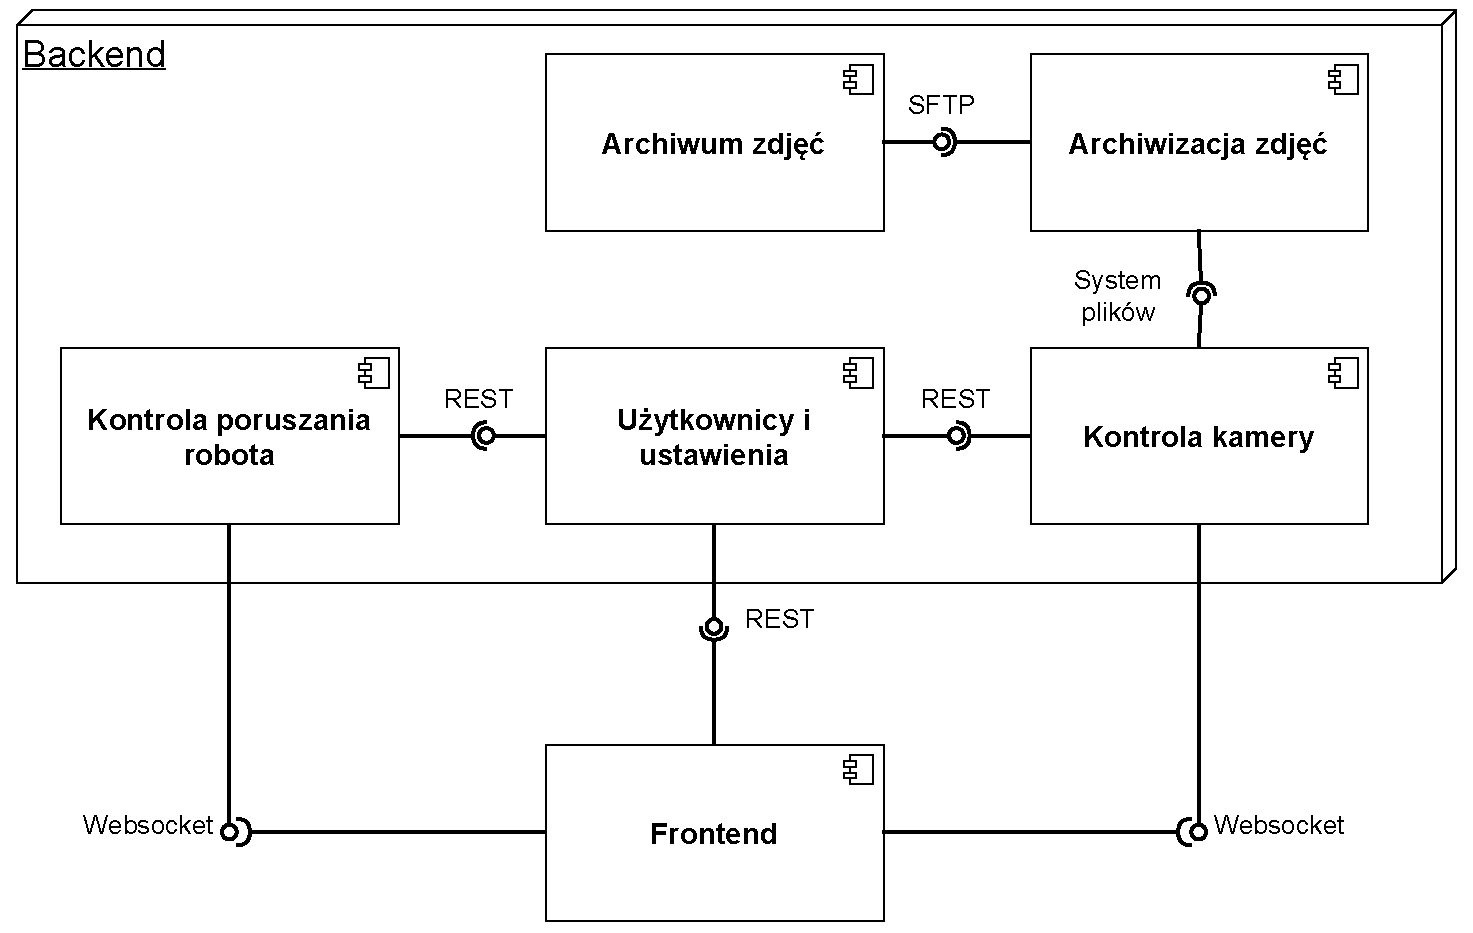
\includegraphics[width=1.0\linewidth]{robot_components.pdf}
    \caption{Diagram komponentów}
    \label{rys:components}
\end{figure}

\section{Wdrożenie}
Wdrożona aplikacja ma działać na sprzęcie samego robota i na urządzeniach końcowych użytkowników.
Wykorzystując możliwości minikomputera Raspberry Pi stawiany jest na nim serwer backendu i frontendu.
Jedynym wykorzystaniem zewnętrznej infrastruktury jest zewnętrzny serwer na pliki, gdzie archiwizowane są zdjęcia.
Architektura wdrożeniowa przedstawiona jest na schemacie \ref{rys:deploy}.

We wdrożeniu wszystkie moduły backendowe są schowane za reverse proxy, które stanowi odpowiednio skonfigurowany serwer HTTP \href{https://nginx.org/}{\textit{nginx}}.
Do uruchamiania całej aplikacji napisany został skrypt w bashu.
Skrypt ten z kolei jest uruchamiany przez specjalnie napisany serwis \textit{systemd}\footnote{\textit{systemd} to menadżer systemu i usług w wielu dystrybucjach systemu operacyjnego GNU/Linux.}.

Jeśli chodzi o architekturę sieciową, to robot jest połączony do internetu przez bezprzewodową sieć Wi-Fi.
Ponadto, administrator może podłączyć maszynę do wirtualnej sieci prywatnej.
\href{https://www.zerotier.com/}{\textit{ZeroTier}} jest popularnym tego typu oprogramowaniem wykorzystanym w tym projekcie.
Dzięki temu rozwiązaniu użytkownicy robota mogą korzystać z systemu robota w jakimkolwiek miejscu z dostępem do internetu.
Jednocześnie \textit{ZeroTier} szyfruje cały ruch sieciowy od końca do końca, co gwarantuje bezpieczeństwo i prywatność.
\begin{figure}[!hb]
    \centering 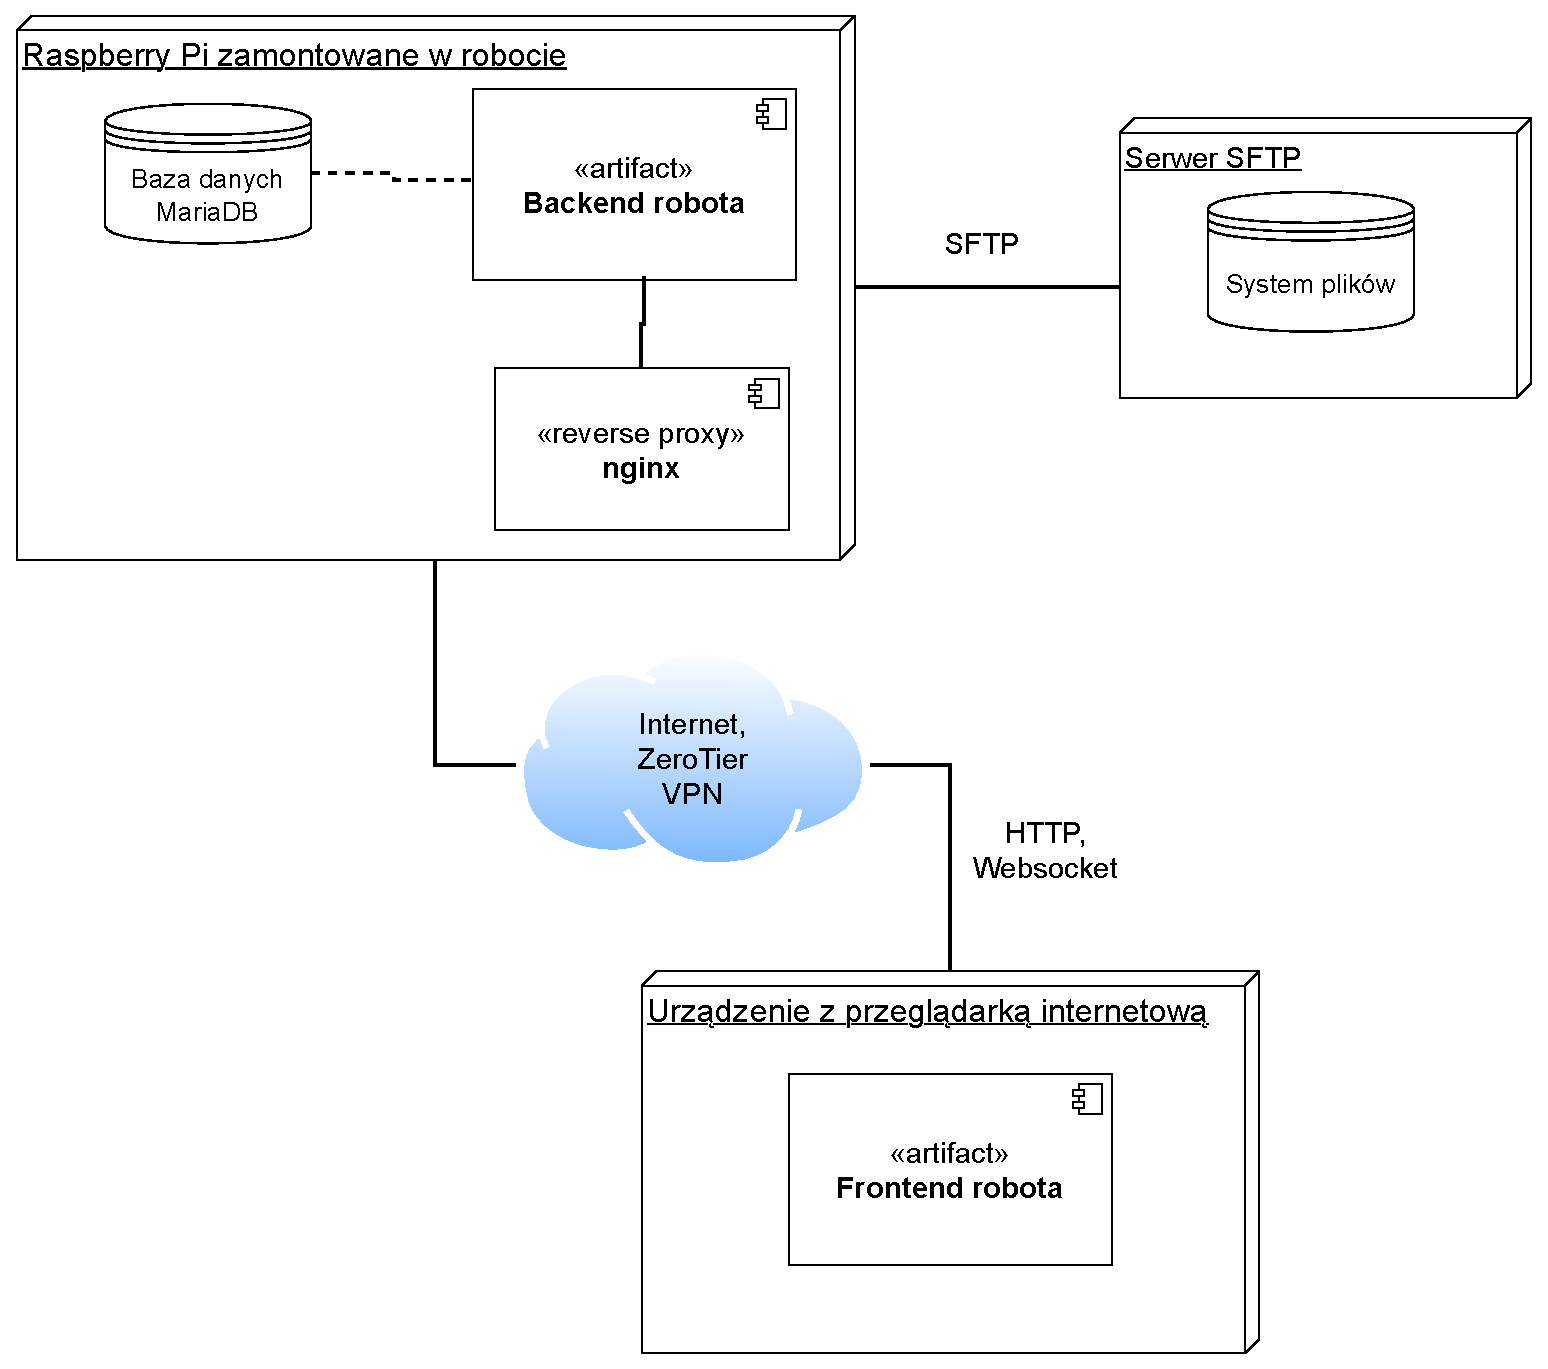
\includegraphics[width=1.0\linewidth]{robot_deploy.pdf}
    \caption{Diagram wdrożenia}
    \label{rys:deploy}
\end{figure}


